\documentclass[notitlepage]{report}
\usepackage[left=1in, right=1in, top=1in, bottom=1in]{geometry}

%Para usar colores en las tablas:
\usepackage{color}
%\usepackage{graphicx} DUPLICADO
\usepackage{epsfig}
\usepackage{multirow}
\usepackage{colortbl}
\usepackage[table]{xcolor}
%Fin de paquetes para usar colores en las tablas


\usepackage{titling}
\usepackage{lipsum}
\usepackage{mathtools}
\usepackage{amsmath}
\usepackage{amsfonts}
\usepackage{amssymb}
\usepackage{pdfpages}
\usepackage[spanish]{babel}
\usepackage[utf8]{inputenc}
\setlength{\parskip}{2mm}
\usepackage{graphicx}
\usepackage{hyperref}
\graphicspath{ {./Imagenes/} } 

%Definiendo colores:
\definecolor{lightgray}{gray}{0.9}
\definecolor{myblue}{RGB}{180,241,231}
\definecolor{myred}{RGB}{241,121,108}
\definecolor{myyellow}{RGB}{245,239,122}
%Fin de definicion de colores:


\pretitle{\begin{center}\Huge\bfseries}
	\posttitle{\par\end{center}\vskip 0.5em}
\preauthor{\begin{center}\Large\ttfamily}
	\postauthor{\end{center}}
\predate{\par\large\centering}
\postdate{\par}

\title{Kurt Bizarre Contact I: Fast TPI and DI Exposition \\ \Large{English/Español}}
\author{Juan Carlos Caso Alonso}
\date{\today}
%\date{19 January/Enero 2023}

%\renewcommand{\chaptername}{C.-}
%\usepackage{fancyhdr}

\addto\captionsspanish{\renewcommand{\chaptername}{C.-}}

\begin{document}
	\maketitle
	\thispagestyle{empty}
	
	\newpage
\renewcommand{\abstractname}{Abstract English}
\begin{abstract}
	\noindent
	Contact letter and exchange of opinions with the account Kurt Bizarre (Samuel). He asks me to define DI and TPI and also to indicate the errors in the demonstrations of the Theorems: \\
	$|A| < |P(A)|$ \\
	$|P(N)| = |R|$ \\
	The second one does not pose any problems since if all infinite cardinals are equal, it is compatible with my statement. And I myself proved it to myself by applying LJA Constructions and the Naive Theorem CA (patience, it's not the time for that today) \\
	
	\noindent
	Expected delivery date is April 18, 2023, as always, I think it will be two pages... and it will be done soon...\\
	
	\noindent
	If you are wondering why this has an abstract, it's because I have a Latex skeleton that I don't know how to change hahahaha, and in English by ChatGPT because I have an American friend to whom I'm going to pass it on, who has been asking me for translated material for a while.
	
\end{abstract}
	\newpage
\renewcommand{\abstractname}{Abstract Español}
\begin{abstract}
		\noindent
		Carta de contacto e intercambio de pareceres con la cuenta Kurt Bizarre (Samuel). Me pide que le defina la DI y la TPI, y que de paso le indique los fallos en las demostraciones de los Teoremas:\\
		1) $|A| < |P(A)|$\\
		2) $|P(N)| = |R|$\\
		El segundo no da problemas puesto que si todos los cardinales infinitos son iguales, es compatible con mi afirmación. Y yo mismo me lo demostré a mi mismo aplicando Construcciones LJA y el Naive Theorem CA (paciencia, hoy no toca eso)\\\\
		
		\noindent
		Fecha de supuesta entrega 18 Abril 2023, como siempre, pienso que son dos páginas... y que se hacen pronto...\\\\ 
		
		\noindent
		Si te preguntas por qué tiene abstract esto es porque tengo un esqueleto de Latex que no se cambiar jajajajaja, y en inglés de chatGPT pq tengo un amigo americano al que se lo voy a pasar, que lleva tiempo pidiéndome material traducido. 
		
	
\end{abstract}
	
	\addtocontents{toc}{\hspace{-7.5mm} \textbf{Capítulos}}
	\addtocontents{toc}{\hfill \textbf{P\'agina} \par}
	\addtocontents{toc}{\vspace{-2mm} \hspace{-7.5mm} \hrule \par}
	
	\tableofcontents
	
	\part{Part I: English}
	
	\chapter{Introduction}
	\chapter{Fast and simple analogy about the fail in the logic of the proofs}
	
	\section{The Table}
	\begin{table}[h!]
		\begin{tabular}{|c|c|c|c|c|c|}
			\hline
			$O\_o!!$ & $R_{1}$ & $R_{2}$ & $R_{3}$ & $R_{4}$ & $R_{5}$ \\
			\hline
			$A$ & $B_{1}$ & $B_{2}$ & $B_{3}$ & $B_{4}$ & $B_{5}$ \\
			\hline
			\hline
			$1$ & $\{1\}$ & $\{1\}$ & $\{1\}$ & $\{1\}$ &$\{1\}$  \\
			\hline
			$2$ & $\{2\}$ & $\{2\}$ & $\{2\}$ & $\{2\}$ &$\{2\}$\\
			\hline
			$3$ & $\{3\}$ & $\{3\}$ & $\{3\}$ & $\{3\}$ &$\{3\}$\\
			\hline
			$4$ & $\emptyset$ & $\{4\}$ & $\{5,6\}$ & $\{4,5,6\}$ & $b=\{a \in A | a \notin R_{5}(a) \}$ \\
			\hline
			$5$ & $\{6\}$ & $\{6\}$ & $\{6\}$ & $\{6\}$ &$\{6\}$\\
			\hline
			$6$ & $\{5\}$ & $\{5\}$ & $\{5\}$ & $\{5\}$ &$\{5\}$ \\
			\hline 
		\end{tabular}
	\end{table}

	\input{./Cap_II_PreviousContext_ENG.tex}
	%DI, TPI, y el fenómeno actual que me está sucediendo
\chapter{Di, TPI and the actual phenomenon that is happenning right now}
	
	Text
	
	\section{DI}
	
	Text
	
	\section{TPI}
	
	
	
	\section{Incredible result}
	%\input{CAPITULOS/Part_I_English/Appendix_1_Optative_Extensions/Appendix_I_EN_OEs.tex}
	
	\part{Parte II: Español}
	
	\chapter{Introducción}
	\noindent
	Lo que me pides... ¿Cuáles serían las palabras: 'No es justo´? No solo me ha costado 25 años desarrollar el contraejemplo, con cada punto chequeado por otra gente y con referencias de dos matemáticos. Encima me pides que te diga el fallo de la demostración, cuando el teorema 1, ($|A| < |P(A)|$), no admite excepciones del tipo $ |\mathbb{N}| = |P(\mathbb{N})| $.\\\\
	
	\noindent
	Es una trampa circular por varios motivos:\\\\
	1) Tengo que resumir y descartar material, MUCHO, porque tengo una ventana de atención por tu parte muy reducida respecto a lo que necesito en realidad. No puedo hacerlo en el formato que me resulta más... 'eficiente´. Y no puedo cometer ni el más mínimo fallo. Y es un campo de minas, y te pido perdón de antemano, porque también debo evitar que 'cortocircuites´. Pensarás que soy un flipado, que soy un ignorante y que digo eso porque no entiendo las críticas que me hacen, pero no es el caso. Como dudo de todo, hasta de mi mismo, suelo usar el feedback que me dan, y descubro 'reacciones curiosas´ cuando unos matemáticos me dicen lo que piensan sinceramente, sobre lo que me dicen OTROS matemáticos... pensando que son ideas mías. Tengo muchísimas anécdotas, de diferente índole.\\\\
	2) Necesito el contraejemplo para que entiendas el fallo de la lógica. Como ya te dije, tengo tiempo reducido y NO puedo explicarte TODO lo que tengo, y no me vas a creer si solo te menciono la existencia de lo que es una 'paradoja híbrida´... :D... Me la voy a jugar, pero... ¿A que te estás preguntado que coño es una paradoja híbrida? :D... Tienes que verlas 'actuar´ para creer que existen. PERO no me dejas usar el contraejemplo completo (4 horas y media delante de una pizarra), y como muchos antes, me pides que te explique el fallo de la demostración, que es, PRECISAMENTE, el contraejemplo (entre otros, pero que tampoco sirve de nada decírtelos si no ves como falla el teorema con tus propios ojos).\\\\
	3) El contraejemplo SÉ que lo tengo más que doblemente chequeado. La explicación del fallo no. No paro de pedir ayuda y no la consigo, a pesar de los resultados que ofrezco. VOY A INTENTAR crearte una 'analogía´ más sencilla y rápida del caso real, PERO RECUERDA, el fallo en la lógica de la demostración, y el contraejemplo, están relacionados, \textbf{\underline{PERO NO SON LO MISMO}}. Puedo construirte relaciones, pero igual meto la pata en terminología de lógica.\\\\
	
	\noindent
	Te pido que no olvides que me dejo mogollón de cosas en el tintero. La TPI tiene mogollón de propiedades, pero no te las voy a decir porque el documento donde me explayé tiene 60 páginas. A Don Pepe Mendez, tardé hora y media delante de una pizarra en explicársela:\\
	https://vixra.org/abs/2209.0120\\
	No me hagas lo que me hizo una persona anteriormente. Primero alucinó con que se pudiesen construir. Luego vino a los dos días y me dijo: mira, puedo construir una entre $\mathbb{Q}$ y $\mathbb{R}$, y como sabemos que ambos tienen cardinal diferente, es irrelevante que existan las TPIs... Lo primero es que YO acepto que se puedan aplicar a $\mathbb{Q}$ y $\mathbb{R}$, ya que tienen el mismo cardinal y es una técnica que nace con intención de generalidad. Básicamente me dice que puede replicar mis resultados y que eso está mal :D. SEGUNDO, no sé si lo has visto pero eso es un argumento circular. Usa el Teorema, para negar un contraejemplo del teorema, para evitar juzgar las repercusiones y las propiedades de las TPIs... por eso te digo que la gente 'cortocircuita´. Si pudiésemos usar un teorema, para negar cualquier contraejemplo, sin más argumentos, se podría demostrar cualquier cosa, pues siempre te puedo decir que lo tuyo es irrelevante ya que el Teorema es cierto.\\\\
	
	\noindent
	Te puedo decir que soy el hombre más guapo del mundo. Th :D. Y tú me puedes enseñar una foto de Brad Pitt. Así que te respondo: ¿Sabes qué, como ya sabemos que soy el hombre más guapo del mundo, ni siquiera le vamos a enseñar esa foto a mi novia, y la vamos a quemar, okey?\\\\
	
	\noindent
	Vamos con la analogía rápida de un caso más sencillo que el real.
	
	
	\chapter{Analogía rápida del fallo lógico de las demostraciones}

	\section{La Tabla}
	\begin{table}[h!]
		\begin{tabular}{|c|c|c|c|c|c|}
			\hline
			$O\_o!!$ & $R_{1}$ & $R_{2}$ & $R_{3}$ & $R_{4}$ & $R_{5}$ \\
			\hline
			$A$ & $B_{1}$ & $B_{2}$ & $B_{3}$ & $B_{4}$ & $B_{5}$ \\
			\hline
			\hline
			$1$ & $\{1\}$ & $\{1\}$ & $\{1\}$ & $\{1\}$ &$\{1\}$  \\
			\hline
			$2$ & $\{2\}$ & $\{2\}$ & $\{2\}$ & $\{2\}$ &$\{2\}$\\
			\hline
			$3$ & $\{3\}$ & $\{3\}$ & $\{3\}$ & $\{3\}$ &$\{3\}$\\
			\hline
			$4$ & $\emptyset$ & $\{4\}$ & $\{5,6\}$ & $\{4,5,6\}$ & $b=\{a \in A | a \notin R_{5}(a) \}$ \\
			\hline
			$5$ & $\{6\}$ & $\{6\}$ & $\{6\}$ & $\{6\}$ &$\{6\}$\\
			\hline
			$6$ & $\{5\}$ & $\{5\}$ & $\{5\}$ & $\{5\}$ &$\{5\}$ \\
			\hline 
		\end{tabular}
	\end{table}

	\section{Explicación de la tabla}
	
	\noindent
	La tabla representa un 'asedio´ a una paradoja híbrida, muy simple. Son cinco relaciones\footnote{
		RARAMENTE voy a usar la palabra 'función´, primero porque es correcto llamarlas también relaciones, antes de ser función debes ser relación. Segundo porque mi trabajo se basa en relaciones que NO son aplicación (recuerda, todo está chequeado, lo hago de forma correcta hasta los puntos débiles que te mencioné en el documento de tres páginas): 
		$\href{https://docs.google.com/document/d/1DwgidmjAFIlmpDw0rucYLSeTMFiOuFxfVQxPFC-6vwI/edit?usp=share_link}{Documento}$
	}. De $R_{1}$ a $R_{5}$ son relaciones entre A, que tiene cardinal 6, y conjuntos de subconjuntos de A, los $B_{i}$, con cardinal 6, también. Cada columna, después de la doble línea, representa los elementos de cada conjunto. La tabla indica que el elemento del conjunto $B_{i}$, está relacionado mediante $R_{i}$, con el elemento de A que está en la misma fila.\\\\

	\noindent
	No sé por qué la gente reacciona airadamente al ver este ejemplo, pero necesito que sea simple para que se vea muy claro varias cosas. Sé de sobras que los conjuntos implicados sólo tienen cardinal 6, y que no son $\mathbb{N}$ ni $P(\mathbb{N})$. Te dije que sería una analogía con un caso más simple.\\\\
	
	\noindent
	Podríamos demostrar que $B_{5}$ NO es sobreyectiva, si 'confiamos´ en la técnica de Cantor. Al crear el par $(4, b)$ en $R_{5}$ creamos la doble contradicción que es núcleo de su demostración (junto con la definición de 'b´). Y a la misma vez, sabemos, gracias a que es muy simple el ejemplo, que A y $B_{5}$ tienen el mismo cardinal. Finito, pero el mismo cardinal.
	
	\noindent
	La demostración habla de 'cualquier relación/función posible entre A y P(A)´, y aquí tenemos un caso EXTREMADAMENTE particular, donde la conclusión de la demostración, cojea. Okey, no son esos conjuntos, pero tienen el mismo cardinal, permiten definir 'b´ y generar la doble contradicción. \\\\
	
	\noindent
	No solo eso. Y esta es la parte del 'asedio´. $B_{5}$ es uno de los otros $B_{i}$ por narices: o es $B_{1}$, o $B_{2}$, o $B_{3}$, o $B_{4}$. Ya que la definición de 'b´ DEBERÍA coincidir con 'alguno´ de los elementos que están en su misma fila, el resto de elementos son idénticos. Eso \textbf{\underline{SI}} 'b´ EXISTIESE y fuese un subconjunto de A. Esto implica que $R_{5}$, en realidad, es una de las otras $R_{i}$... que no generan dobles contradicciones y sí son biyectivas.\\\\
	
	\noindent
	Fíjate lo curioso que es: al cambiar la definición del subconjunto hemos desactivado la doble contradicción, pero usando EL MISMO subconjunto. No pasa nada por crear los pares:\\
	$(4, \emptyset)$, \\ 
	$(4, \{4\})$,     \\
	$(4, \{5,6\})$ y  \\
	$(4, \{4,5,6\})$  \\
	Lo malo es que no sabemos exactamente CUAL de ellos es 'b´, y a la misma vez, debe ser alguno de ellos. YO, no lo tengo claro, al menos :D. Pero gracias a que el ejemplo es tremendamente sencillo, sabemos con certeza que de $R_{1}$ a $R_{4}$ son todas relaciones, funciones, biyectivas.\\\\
	
	\noindent
	¿Lo experimentas? Este es el sabor de boca que te deja un asedio para atacar una paradoja híbrida. Claro, en su versión light. Yo estuve sin dormir tres días... pero igual tú te libras. Otra gente se cabrea. O cortocircuita.\\\\
	
	\subsection{Punto 1}
	
	\noindent
	No sé como expresar esto de forma 'formal´: las diagonalizaciones son IRRELEVANTES, pq se pueden construir sobre conjuntos con el mismo cardinal. Pero esa afirmación no me la he sacado de la manga, como me hicieron con la TPI, que SI busca poder crearse entre conjuntos con... 'el mismo cardinal infinito´. Con una simple observación de la tabla puedes coincidir conmigo: los elementos de cada conjunto se pueden contar a ojo, si hubiese dudas :D.\\\\
	
	\subsection{Punto 2}
	
	\noindent
	2) Me dirás que me queda la de $\mathbb{N}$ vs $\mathbb{R}$ ( o cadenas binarias infinitas representando el conjunto de Cantor), que no me la has pedido. El Teorema 2 de tu lista:\\
	$|P(\mathbb{N})| = \mathbb{R}$\\
	No contradice mis afirmaciones. Y este que te sugiero lo tengo analizado en estas dos horas de vídeos de youtube:\\
	\href{https://www.youtube.com/watch?v=reRUUKGFXf0&list=PLcEv5UNDUdw68yFXf2kYGDZVyIGpCfGdy}{Lista de videos}\\
	TE ADVIERTO, mi material es caótico. Solo te lo pongo para que 'tengo algo para eso´. He aprendido a ordenarlo un poco todo y lo estoy reescribiendo. Esos vídeos necesitan unos pequeños apaños. Es una rama no chequeada todavía. Se repiten montón de cosas porque hay que explicar las definiciones y propiedades comunes en cada rama, si empiezo de cero con alguien... Te vas a quedar a cuadros, pero básicamente puedo PREDECIR cualquier elemento externo, creado con cualquier técnica de diagonalización, CUALQUIERA, para cualquier intento de biyección POSIBLE entre $\mathbb{N}$ y $P(\mathbb{N})$, con relaciones PREVIAMENTE establecidas. ¿Qué apaños?¿Qué significa 'predecir´?¿Cómo que uso más de una relación?... :D. Por eso sólo quiero decirte que 'existe´.
	
	\noindent
	\textit{NOTA: perdona que me ponga quizás prepotente. Sé que hay más demostraciones... YO NO SOY matemático. UN SOLO contraejemplo las invalida TODAS. Mencionarlo es indigno de un matemático de carrera. Es mucho morro pedirme que arregle TODAS. YO SOLO. Ni siquiera las conozco. He visto alguna y 'creo´ saber por dónde van los tiros del error... pero una vez más, no paro de pedir ayuda, y como no soy nadie... pues eso.}\\\\
	
	\noindent
	Salta aquí al punto 3, el resto de esta subsección solo lo escribo para dejar constancia. Necesitas mogollón de contexto para entender los apaños, aunque, por si los lees, trataré de explicarte 'algo´.
	
	\subsubsection{Añadido ignorable solo para dejar constancia}
	
	Texto
	
	\subsection{Punto 3}
	
	\noindent
	Ya sé, ya sé... el ejemplo es demasiado sencillo. PERO, si ya se dá en UN caso ¿Sucederá en más? Y la gracia es que sucede para $\mathbb{N}$ vs $P(\mathbb{N})$.\\\\ 
	
	\noindent
	En este ejemplo se vé fácil porque los conjuntos son muy sencillos. El asedio sólo consiste en crear todas las alternativas posibles a la función característica de 'b´, con descripciones que solo listan directamente los elementos. Cambiamos su función característica, SIN CAMBIAR el subconjunto final: 'alguna de ellas´ es una función característica\footnote{Espero no equivocarme. La función que dice si un elemento pertenece o no al conjunto} equivalente a la de 'b´. Las dos generan el mismo subconjunto de A.\\\\
	
	\noindent
	En el caso real, no solo vamos a cambiar TODAS las funciones características de TODOS los elementos de $P(\mathbb{N})$. Vamos a crear alternativas al concepto de 'función´ (relaciones no aplicación que van a ser 'útiles´), al concepto de inyectividad o biyectividad para comparar cardinalidades infinitas, vamos a poner en duda la definición de 'cardinalidad´... e incluso puede que algún axioma ZF... vamos a 'intuir´ que existen fenómenos lógicos nuevos (las Paradojas Híbridas\footnote{Una P.H. es un absurdo metido con calzador, que es un absurdo en sí mismo, al ser paradoja, que en realidad no está relacionado con la frase original de la demostración. Para pequeña muestra, un pequeño botón... $R_{5}$ debería ser biyectiva, a pesar de la doble contradicción que podemos generar gracias a la definición de 'b´. Se llaman híbridas, pq tienen muchos estados diferentes, según la relación de la que dependen, es un buen subconjunto, o se convierte en paradoja... y nos permite decir que hemos llegado a un absurdo, cuando lo único que hemos hecho es añadir una paradoja por la cara en mitad de la demostración}). Y lo que no me esperaba, vamos a expandir el asedio a dos técnicas diferentes. Cuando presento la TPI, para negarla, me GARANTIZAN justo el punto que me faltaba de la DI, y para negar la DI, me GARANTIZAN justo el punto que me faltaba en la TPI. ¿Cuál de las dos es la correcta? ASEDIO!! Jajajaja. Las dos dependen de interpretaciones complementarias del mismo tipo de intersecciones infinitas... para cada posible interpretación, tengo una construcción de 'equivalente´ a una relación inyectiva imposible según Cantor. Aunque no sepa decirte cuál es la interpretación correcta de las dos.\\\\

	\noindent
	¿Se pueden construir diagonalizaciones? Sí, pero si no me das 4 horas y media, me niegas el contraejemplo, me niegas el poder enseñarte el equivalente a poder ver que todos los conjuntos implicados SIEMPRE han tenido cardinal 6 (en el ejemplo de la tabla).\\\\
	
	\noindent
	No nos podemos saltar el orden. Para que entiendas el fallo de las demostraciones, necesito enseñarte el contrajemplo primero. Esa es mi serpiente que se muerde la cola.	Todo el mundo me insiste en que si el contraejemplo existe, les indique el fallo de las demostraciones. Y eso es imposible, al menos para mí. NECESITO el contraejemplo. Debes entender que las diagonalizaciones son irrelevantes y que petan de muchas maneras diferentes si las estudias a fondo.
	\\\\
	
	\noindent
	\textit{Aquí ya me meto droga dura en vena: no me hagas mucho caso :D. Una paradoja híbrida no es una función característica válida de un subconjunto, no es un Teorema, y no es un programa (Cantor, Gödel, Turing...). Por eso hay que cambiar un axioma de ZF, para añadir de alguna manera la coletilla de que no puede crearse un subconjunto con una paradoja híbrida. Hay que estudiarlas a fondo, para mejorar su detección y definición, por si también afectan a los teoremas de Gödel, Turing... y alguno de Teoría de Lenguajes Formales. O por si hay más casos...}\\\\
	
	

	
	
	
	
	
	
	
	




	\chapter{Intento de Contexto Previo Mínimo}

	\section{Relaciones no aplicación}

	\noindent
	Tanto la TPI como la DI, están basadas en relaciones que no son aplicación: la flja\_abstracta y las diferentes $r_{\theta_{k}}$. En realidad son lo mismo. TODAS son en el sentido:\\
	$r: P(\mathbb{N}) \rightarrow \mathbb{N}$\\
	\textit{* Sí, invierto el orden común... y te estoy mintiendo un poco... para ir rápido... en realidad son ``subconjuntos transformados'' de ellos dos, con sus mismos cardinales, pero esa es otra historia... Me pides cosas concretas, que no siguen el orden natural de exposición, y eso me obliga a saltarme cosas... y adaptarlas para tí y esta carta. En su debido momento deberías autorizar dichas transformaciones, pero ya lo han hecho otros antes que tú. Son correctas. Debes creerme :D, hasta que tengas tiempo de verlo por tí mismo.}
	\\\\
	
	\noindent
	Llamemos:\\
	R-pares: a los pares de las relaciones. ( elemento de $P(\mathbb{N})$, elemento de $\mathbb{N}$ ).\\
	D-pares: a pares creados con elementos del Dominio, o sea $P(\mathbb{N})$. ( elemento de $P(\mathbb{N})$, elemento de $P(\mathbb{N})$ ).
	\\\\
	
	\noindent
	No voy a definirte en este documento la flja\_abstracta, pero es una relación; un conjunto de pares; R-pares. Como conjunto, se le puede hacer una partición. Una partición muy particular, que a parte de otras propiedades, tiene la de generar TODAS las relaciones $r_{\theta_{k}}$. Cada $r_{\theta_{k}}$ es un subconjunto de la flja\_abstracta, disjunta con el resto de relaciones $r_{\theta_{k}}$. No tienen R-pares en común entre ellas. Y me tengo que morder la lengua aquí... para no abrir demasiados melones. La DI real, aplicada, usará la flja\_abstracta, y la TPI, real, aplicada, usará las diferentes relaciones $r_{\theta_{k}}$ sin hacer trampas con el cardinal de $\mathbb{N}$ (otra cosa es que haga ``trampas'' dentro de cada $r_{\theta_{k}}$). En realidad solo estaremos hablando de una redistribución de R-pares :D.
	\\\\
	
	\noindent
	Como las relaciones no van a ser aplicación, van a haber elementos del Dominio con más de una imagen. No vamos a crear los pares así:\\
	( $SUBCONJUNTO_{i}$, $\{n_{0}, n_{1}, ..., n_{j} \}$ )\\
	Sino así:\\
	( $SUBCONJUNTO_{i}$, $n_{0}$ )\\
	( $SUBCONJUNTO_{i}$, $n_{1}$ )\\
	...\\
	( $SUBCONJUNTO_{i}$, $n_{j}$ )\\
	Todos los elementos del Dominio ( $P(\mathbb{N})$ ), en TODAS las relaciones, van a existir en al menos UN R-par. Vamos, que van a tener imagen, aunque haya que repetir el uso de algunos elementos de $\mathbb{N}$.
	\\\\
	
	\noindent
	Sí, keep calm, van a haber D-pares que usan el mismo $n \in \mathbb{N}$, para ambos miembros del D-par, en algunos R-pares de esa relación. A eso lo llamaremos una 'repetición´.
	\\\\
	
	\noindent
	Curiosamente, llamáis igual al conjunto Imagen de cada elemento del Dominio, y al conjunto Imagen de la relación (que hay varias, ojo, :D). El conjunto Imagen de un elemento del Dominio, estará formado, una vez estudiados TODOS los R-pares de esa relación, por todos los $n \in \mathbb{N}$, que aparezcan con él, en algún R-par.
	\\\\
	
	\noindent
	Un 'PACK´ de un elemento del Dominio, según una relación r, es un subconjunto, propio o impropio, de su conjunto Imagen. No solo les cambio el nombre para diferenciarlos, sino porque pueden tener incluso diferentes cardinales para cada elemento.
	
	
	\section{NAIVE CA theorem, sin demostración}
	
	\noindent
	1) Si podemos construir una relación\\
	$r: A \rightarrow B$\\
	Siendo A y B conjuntos con cualquier cardinalidad, finita o infinita.
	\\\\
	
	\noindent
	2) Donde para cada elemento de A, en base a los R-pares de r:\\
	2a) Podamos crear un PACK con cardinal mayor que 0, distinto de vacío.\\
	2b) Siempre mantengamos el mismo PACK para el mismo elemento del Dominio.\\
	2c) Todos los PACKs creados, para todos los elementos de A, sean disjuntos entre sí.
	\\\\
	
	\noindent	
	3) ENTONCES: Podemos afirmar que $|A| \ngtr |B|$
	
	
	\subsection{Apreciaciones}\part{title}
	
	\noindent
	\textbf{I)} Ojo al dato: tu estás acostumbrado a buscar igualdad, yo me voy a obsesionar con demostrar que el cardinal de uno, NO es mayor que el cardinal del otro, por cualquier herramienta posible. Si no existe, me la invento :D... previo acuerdo de que la herramienta sea ``legal'' matemáticamente. Ya sabemos que $|\mathbb{N}|$ no ``es mayor'' que $|P(\mathbb{N})|$. Demostrarlo a la inversa es una versión cutre, pero efectiva, del teorema Cantor-Bernstein-Schröder. Decir ``NO es mayor'' deja una puerta abierta a la igualdad. Una de mis anécdotas es explicarle esto a un matemático... que corrió demasiado al suponer. Ya no recuerdo quién fue, me dijo: ``Eso está mal, porque pueden ser iguales''. El gatillo del ``eso está mal'' lo tienen muy sensible. No me molesta, si se me permite responder, y mientras la gente no se ofenda porque les corrija alguien como yo.\\\\
	
	\noindent
	\textbf{II)} Otra forma de verlo, es pensar en conseguir que todos los D-pares, tengan PACKs disjuntos en la relación r. Pero siempre eligiendo el mismo PACK, para el mismo elemento del Dominio, da igual en que D-par aparezca. Eso nos lleva a una similitud con la definición de inyectividad:\\\\
	Dada $f: A \rightarrow B$\\
	Y\\
	$f(a_{1}) = f(a_{2}) \leftrightarrow a_{1} = a_{2}$, para cualesquiera $a_{1},a_{2} \in A$\\
	Entonces f es inyectiva.\\\\
	
	\noindent
	Esta definición nos obliga, de forma indirecta, a estudiar TODOS los D-pares de f. Al igual que el NAIVE CA Theorem, nos obliga a estudiar TODOS los D-pares, de r. Vamos a estudiar Dominio X Dominio. Te vas a hartar de escuchar la palabra 'par´. Por eso tengo que llamarlos de forma diferente.\\\\
	
	\noindent
	\textbf{III)} Cuando todos los PACKs, tienen cardinal 1, es un caso particular del NAIVE CA Theorem, que es una definición alternativa a la inyectividad. YA que la relación se vuelve función (solo hay una imagen por elemento del Dominio), y solo cambiamos decir 'imagen diferente´ por 'imagen disjunta´ :D.\\\\
	
	\noindent
	El NAIVE CA Theorem es una generalización de la inyectividad para relaciones que no son aplicación. La inyectividad es un caso particular del NAIVE CA Theorem. PERO, rigurosamente hablando, el NAIVE CA Theorem no encaja en la definición de biyección. No siempre.\\\\
	
	\noindent
	\textbf{IV)} Por favor, es una tontería, pero recuerda:\\
	$\{7, 23, 5027\}$ y $\{8, 23, 5028\}$\\
	Son diferentes, pero NO disjuntos... no vamos a permitir ni un solo elemento en común entre los PACKs. Es esencial recordar que no vamos a buscar imágenes (PACKs), diferentes, sino DISJUNTAS. Esto viene por si caes en la trampa mental de creer que las relaciones son en realidad entre $P(\mathbb{N})$ y $P(\mathbb{N})$. Si los PACKs son disjuntos... por mucho que cada uno sea subconjunto de $\mathbb{N}$, todos juntos forman una partición de algún subconjunto de $\mathbb{N}$. Cosa que no se puede asegurar si solo fuesen 'diferentes´. 
	
	
	\section{Definición de 'resolver´}
	
	\noindent
	Decimos que una relación r, RESUELVE un D-par, si es capaz de generar PACKs disjuntos para los miembros de ese D-par concreto. Usando siempre, el mismo PACK, para el mismo elemento del Dominio, a la hora de estudiar TODOS los D-pares. Sin cambiarle un solo elemento. Ni de más, ni de menos.
	\\\\
	
	\noindent
	Si el mismo elemento del Dominio, lo observamos en otro D-par... puede que ya no sean disjuntos los PACKs, pq el PACK del nuevo elemento no lo es con el de este.
	\\\\

	\noindent
	RESOLVER, no es una propiedad de elementos aislados, sino de D-pares aislados... un mismo elemento puede estar en otro D-par, y ese D-par no estar resuelto por la relación r. No hay problema, el anterior D-par sigue siendo considerado como resuelto. POR ESO insistiré... nuestro espectro, no van a ser elementos del Dominio, sino de Dominio X Dominio.
	\\\\
	
	\noindent
	Lo idea de cambiar de espectro no es cosa mia, sino de Cantor. La definición de inyectividad te lleva a pensar en ello.
	\\\\
	
	\noindent
	Como penúltima cosa a recordar y precisar. Si dos PACKs, de un D-par concreto, tuviesen tres trillones de elementos cada uno, y SOLO, un elemento en común, no contaría como D-par resuelto por la relación r, sino como 'repetición´.
	\\\\
	
	\noindent
	Si en un D-par, resulta que ambos elementos del Dominio, son el mismo elemento, aunque sus PACKs no sean disjuntos, se considera resuelto. No necesito que sean disjuntos los PACKs si están asignados al mismo elemento.
	\\\\
	\chapter{DI, TPI, y el fenómeno actual que me está sucediendo}

	\noindent
	Ambas, la DI y la TPI, son ``juegos cardinales''. La DI es más vieja y es menos ``rigurosa'' en su exposición. Las dos parten del supuesto, que si el conjunto que hace el papel de Dominio, es ABSURDAMENTE mucho mayor que el otro, si su diferencia cardinal es INCONMENSURABLE, :D, no deberían poder construirse con éxito. Y si se construyen con éxito, ambas implican que el cardinal del Dominio, NO es mayor que el cardinal del otro conjunto (que no tiene por qué ser el conjunto Imagen, ojo). Lo cual implica que pueden ser iguales.

	\section{DI:variante pelea de colegio}
	
	\noindent
	DI significa Diagonalización Inversa. Busca un fenómeno similar a la diagonalización, invirtiendo los papeles conocidos de las cardinalidades $\aleph_{1}$ y $\aleph_{0}$. Da igual que barras todas las opciones disponibles para el Dominio ($\aleph_{1}$), NUNCA podrá 'cubrir´ todos los elementos del conjunto con cardinalidad $\aleph_{0}$.
	\\\\
	
	\noindent
	Consiste en que dos alumnos de un colegio se quieren pelear, comparando la cantidad de amigos que cada uno puede aportar a la pelea. Los amigos de Domenicus (Dominio: D) y los amigos de Luciferio\footnote{Lucifer: portador de Luz, Luz $\rightarrow$ Imagen :D.} (Imagen: I). Domenicus le ha dicho a Luciferio que las paradojas híbridas no existen, y no le deja a Luciferio reproducir el experimento que así lo demuestra\footnote{Déjame descargar frustración en alguna parte...}. Antes de que esta afrenta al honor acabe en un baño de sangre, Luciferio le dice a Domenicus que más le vale rendirse ya que tiene amigos suficientes como para estar en una proporción 2 a 1 o superior.
	\\\\
	
	\noindent
	Domenicus no se fía de Luciferio, tiene fama de tramposo, así que le exige una lista detallada que diga, exactamente, que amigos suyos se van a pelear con cada uno de sus amigos. Así que Luciferio le entrega este esquema (Empecemos por un caso finito, para entender el juego):
	\\\\
	
	\noindent
	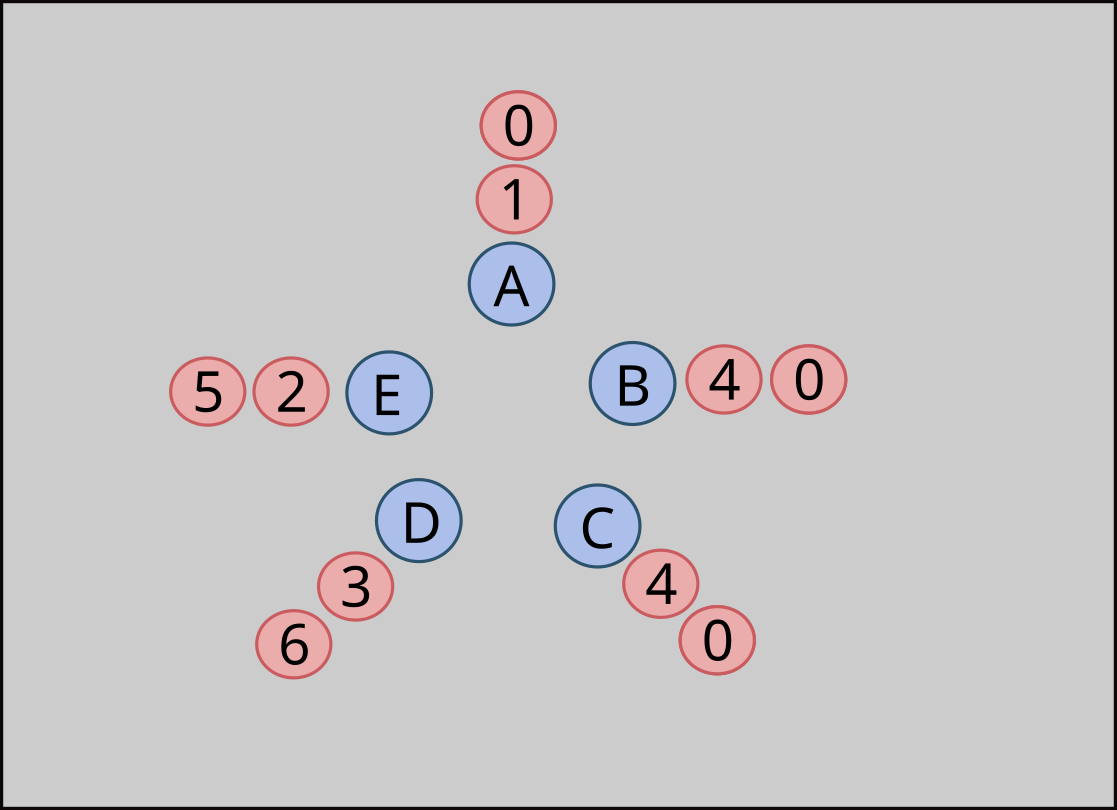
\includegraphics[scale=0.5]{Distribucion_001_A}\\\\
	Como en este colegio son gente muy rara, los amigos de Domenicus tienen nombre de letra, y los de Luciferio tienen nombre de número natural. Vemos que cada amigo de Domenicus(D) tiene un ``Pack'' de amigos de Luciferio(I) asignados. El cardinal de esos Packs es de 2... así que aparentemente Luciferio no mentía con su amenaza.
	\\\\
	
	\noindent
	Después de observar un rato, Domenicus se da cuenta que Luciferio ha hecho trampas: ha puesto a su amigo ``$0$'', dentro del Pack de dos de sus amigos: A y B. Se queja a Luciferio, y este le dice: ``¿Sabes qué, quita a $0$ de la pelea, lo retiro, y si encuentras más repeticiones de uso, también los retiraré de la pelea''. Domenicus luego se fija en que $0$ también está dentro del Pack de C. Luciferio le dice que cuando apartas a uno de sus amigos de la pelea, eso significa quitarlo de TODOS los Packs donde pudiese estar. Así lo hacen y el esquema queda así:\\\\
	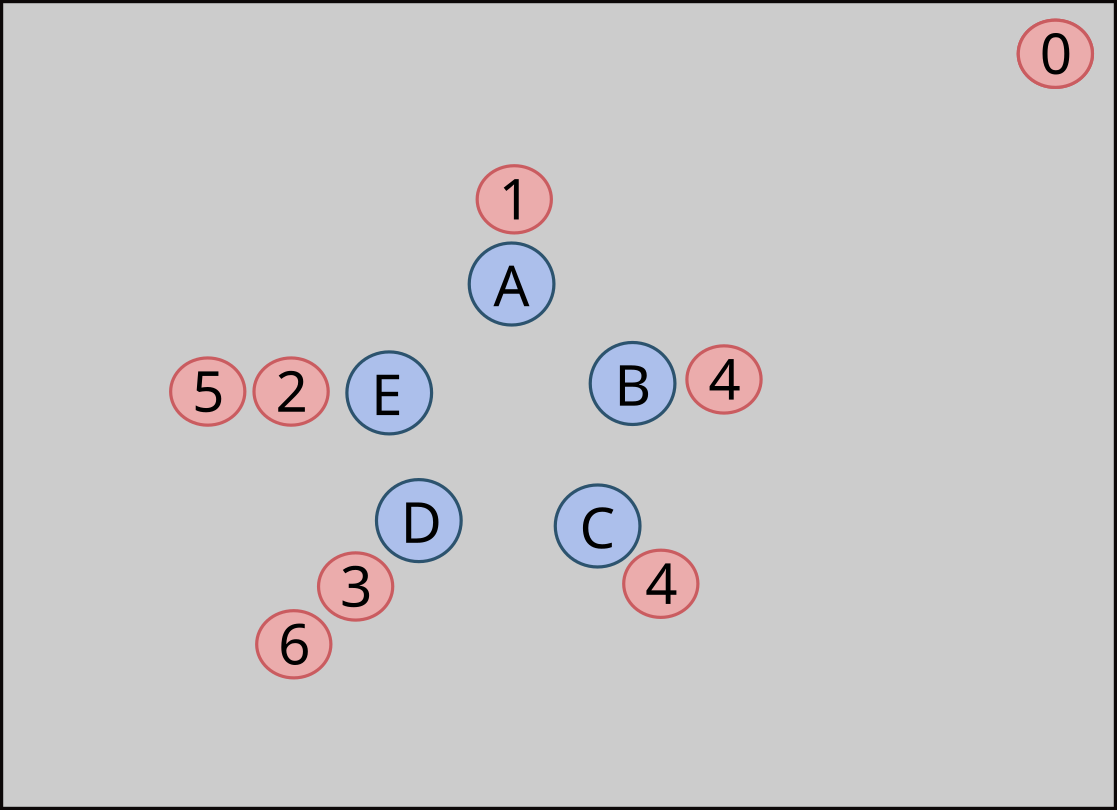
\includegraphics[scale=0.5]{Distribucion_001_B}
	\\\\
	
	\noindent
	Domenicus, que es conocedor de técnicas secretas y avanzadas en teoría de conjuntos, sigue buscando par por par, para ver si Luciferio ha hecho más trampas o si efectivamente, después de descartar a $0$, los Packs nuevos creados a partir del primer esquema (la relación no aplicación original), cumplen las condiciones del Naive CA Theorem.
	\\\\
	
	\noindent
	Domenicus pregunta por el actual estado de los D-pares (E,D), (D,C), (E,A)... (A,B). Los nuevos Packs de (A,B) son más pequeños que los originales, pero ahora son disjuntos, así que este D-par no da más problemas. Y cuando se empieza a desesperar, Domenicus encuentra el D-par (B,C). Tienen el 4 repetido. Siguiendo el acuerdo con Luciferio, 4 se retira de la pelea y lo ``retiran'' de todos los Packs donde pudiese estar:
	\\\\
	
	\noindent
	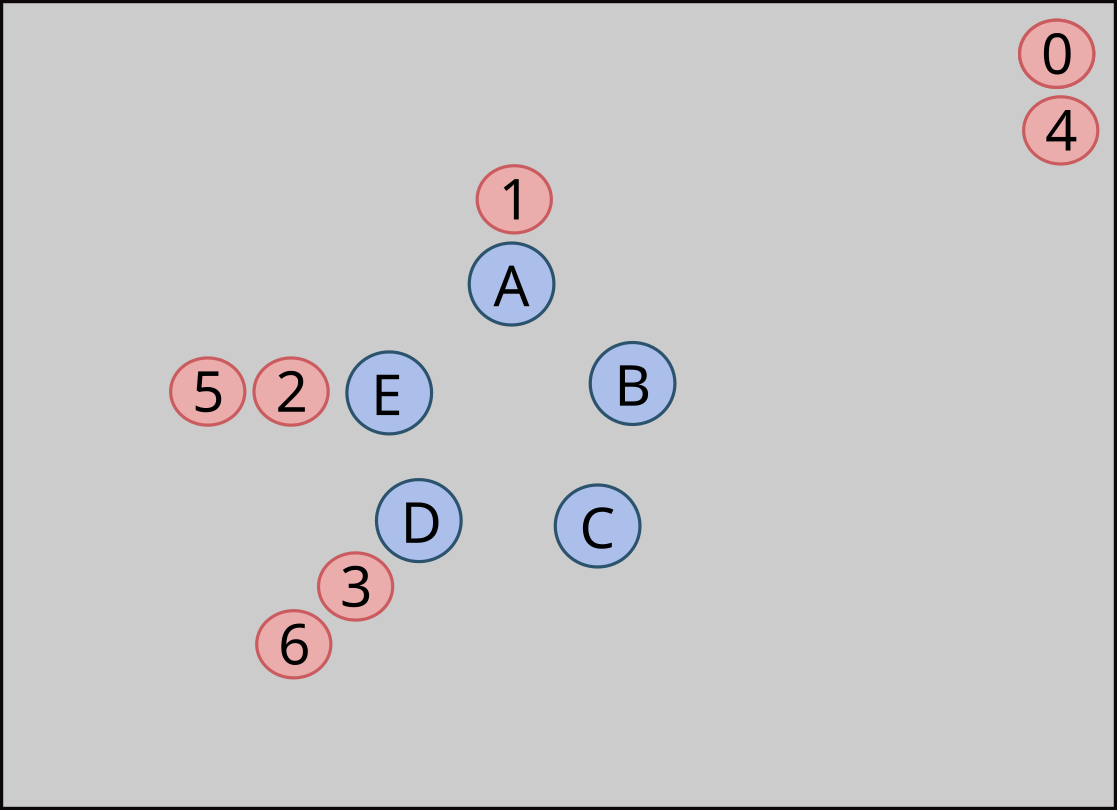
\includegraphics[scale=0.45]{Distribucion_001_C}
	\\\\
	
	\noindent
	Ahora, B y C, tienen Packs asignados completamente vacíos. Domenicus se ríe de Luciferio:``No solo mentiste con la proporción 2 a 1, sino que ni siquiera cumples el Naive CA theorem!!''. Luciferio se enfada mucho, llama a más amigos e intenta otra distribución nueva:
	\\\\
	
	\noindent
	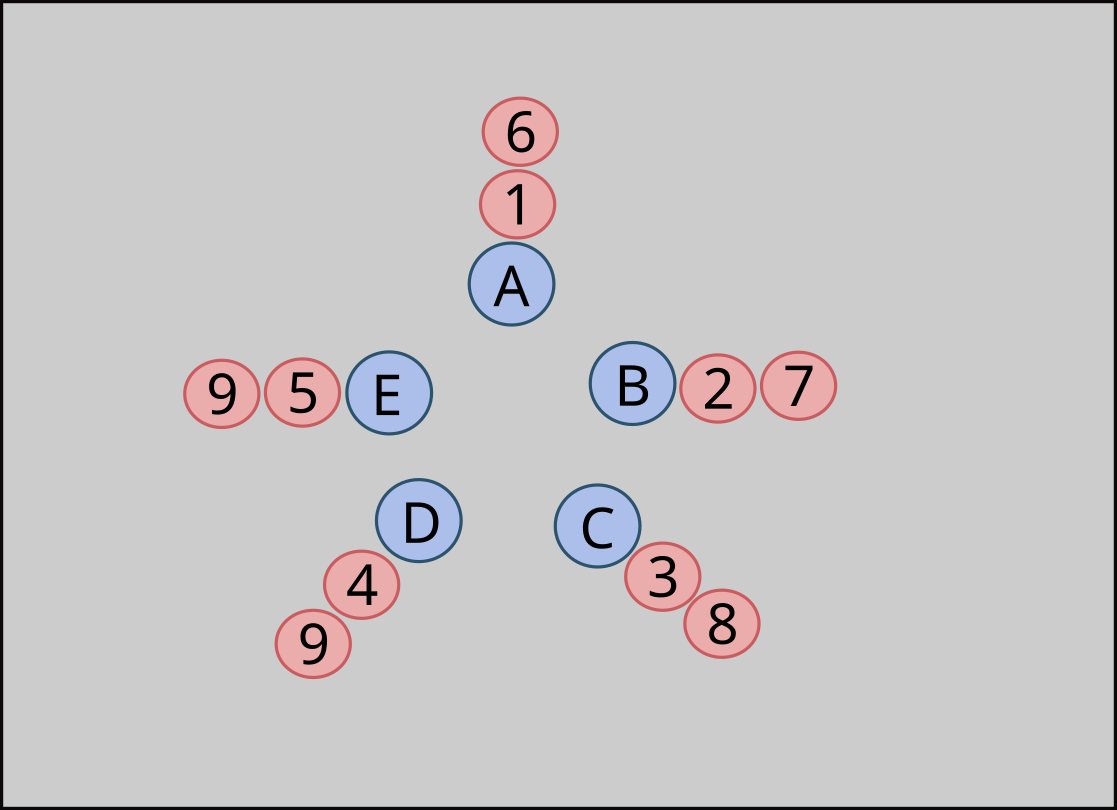
\includegraphics[scale=0.45]{Distribucion_002_A}
	\\\\
	
	\newpage
	

	\noindent
	Rápidamente Domenicus se fija en el D-par (E, D) que repiten el uso del colega 9. Lo apartan y los Packs quedan así:\\\\
	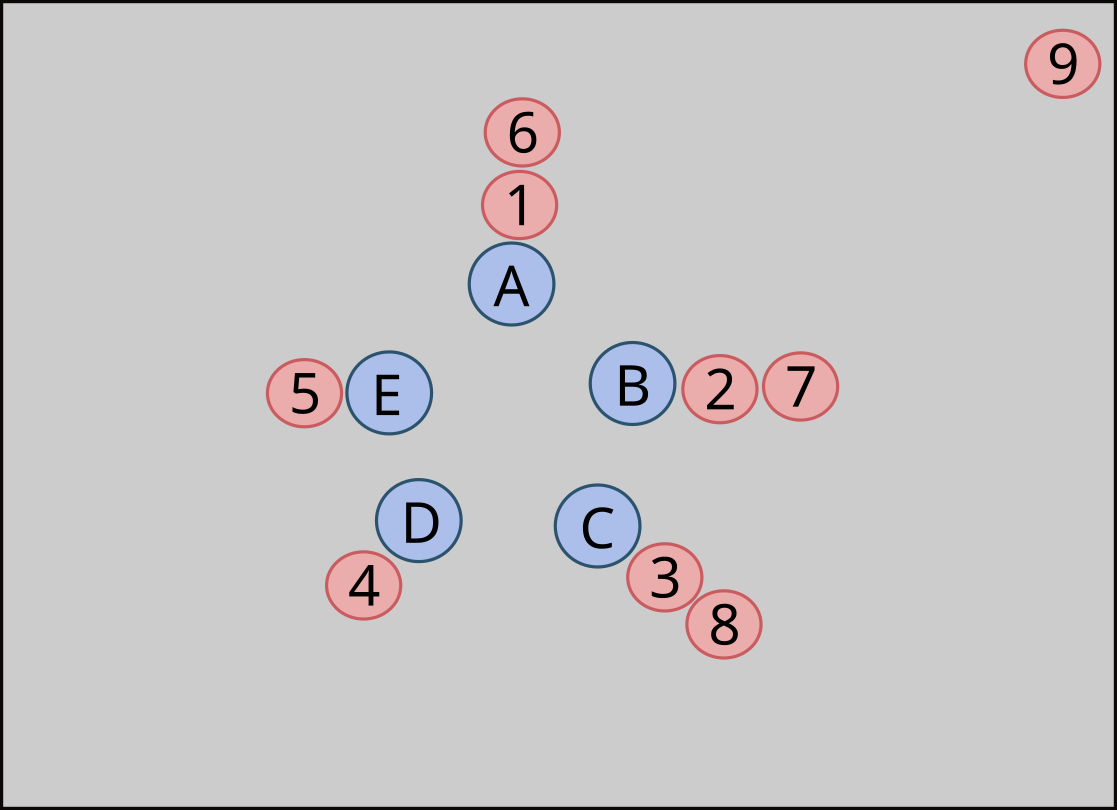
\includegraphics[scale=0.45]{Distribucion_002_B}
	\\\\
	
	\noindent
	Después de este movimiento, Domenicus busca con desesperación otros D-pares con Packs que no sean disjuntos pero ya no encuentra ninguno. La nueva distribución cumple las condiciones del Naive Ca Theorem. Luciferio no cumplió su amenaza totalmente de conseguir una proporción 2 a 1, pero donde no le iguala en número, le supera. Cumplir las condiciones del Naive Ca Theorem indica igualdad de elementos, o algo peor. Se sabe en inferioridad numérica, y aparte debe confiar en que Luciferio no use a sus amigos `` apartados''. Lo cual empeora la inferioridad numérica.
	
	\subsection{Observaciones de la DI}
	
	\noindent
	Partimos de una relación original, posiblemente que no sea aplicación, que está PREDEFINIDA antes de comenzar el juego y que define un conjunto Imagen para cada elemento del Dominio. A partir de ellos, tratamos de ``escoger'' Packs disjuntos, estables, para conseguir cumplir las condiciones del Naive CA Theorem.
	\\\\
	
	\noindent
	Nuestros Packs, comienzan siendo el conjunto Imagen de cada elemento. Según otra persona cualquiera, va escogiendo elementos aleatorios del conjunto Dominio X Dominio, vamos ``recortando''\footnote{A esto lo llamamos en inglés el proceso de ``chopping''} los Packs, eliminando los elementos, no solo de dentro de ellos, sino de cualquier lugar en el que aparezcan en la relación.
	\\\\
	
	\noindent
	No siempre, al preguntar por un D-par, nos obligará a recortar los Packs. A veces, según el orden por el que se pregunte por los D-pares, al preguntar por un D-par concreto, ya habremos eliminado los elementos que impedían a sus Packs ser disjuntos... así que recortar los Packs depende INCLUSO del orden en que recorramos los D-pares.
	\\\\
	
	\noindent
	Si después de haber preguntado por TODOS los D-pares, ninguno de los Packs es vacío, y tienen al menos, un solo elemento, hemos ganado el juego. Cumplimos las condiciones del Naive Ca Theorem:\\
	1) Hay un Pack por cada elemento del Dominio.\\
	2) Cada Pack es No vacío.\\
	3) Todos los Packs son disjuntos entre sí (pq hemos recorrido todos los D-pares y hemos eliminado los elementos que lo impedían).\\
	PODEMOS afirmar que $|Dominio|\ngtr |Imagen|$.
	\\\\
	
	\noindent
	Nuestro ``conjunto especial'' no es uno, sino varios. Son los conjuntos que nos permiten medir el éxito de nuestra labor de forma objetiva. Son los Packs, actuando y sufriendo el ``chopping'' en paralelo. CONSEGUIMOS construir la DI, si algún elemento sobrevive al proceso de ``chopping''. SI NUESTROS CONJUNTOS NO SE VACÍAN. Solo nos hace falta un único elemento, solo uno, por cada Pack (o más). A la misma vez, da igual el éxito del resto, solo un Pack vacío indicará nuestro fracaso. No podremos afirmar nada con seguridad.
	\\\\
	
	\noindent
	El proceso de chopping, se puede definir como una intersección, por cada Pack. Una intersección diferente por cada Pack. Una intersección entre todos los sub-estados de ese Pack. Si el Pack fuese el conjunto $P$, y sus sub-estados, subconjuntos de $P$ llamados $P_{i}$, se cumpliría:\\
	$P_{i+1} \subset P_{i}$\\
	El siguiente estado, en caso de haber un recorte, es el mismo conjunto anterior, pero al que le hemos quitado algunos elementos.\\
	La intersección para cada Pack sería algo así como:\\
	$P_{0} \cap P_{1} \cap P_{2} \cap P_{3} \cap ... \cap P_{final}= ?$
	\\\\
	
	\noindent
	Como los conjuntos infinitos hacen sus locuras, el ÚNICO punto débil de la DI va a ser la interpretación de dichas intersecciones: ¿Si la intersección da un resultado de vacío podemos afirmar que los Packs se vacían? Y esto que parece una pregunta sencilla aparentemente, hay matemáticos que dicen que aunque el resultado sea vacío, no indica ``siempre'' que los Packs se vacían. Otros dicen que ES OBVIO, que si la intersección tiene un resultado INNEGABLE de vacío, indica que los Packs se han vaciado.
	\\\\
	
	\noindent
	La intersección es necesaria porque un proceso secuencial infinito de chopping, NO TIENE FIN... no hay un $P_{final}$. Pero una intersección puede tener términos infinitos, que yo sepa, si estos tienen un cardinal $\aleph_{0}$. Así que nos podemos preguntar por su resultado, y tratar de interpretarlo.
	\\\\
	
	\noindent
	En el futuro de este documento y otros, veremos que el resultado de vacío es inamovible para la flja\_abstracta en el caso $P(\mathbb{N})$ vs $\mathbb{N}$:\\
	a) Si escogemos la interpretación de que los Packs se vacían, El Teorema de Cantor sobrevivirá: nuestros Packs no han conseguido que algunos elementos sobrevivan dentro de ellos, al finalizar el proceso de chopping.\\
	b) NO PODEMOS escoger la opción de que no se vacían en este tipo de intersecciones... sin destruir el Teorema de Cantor. Eso significaría que nuestros Packs sobreviven, y se cumple el Naive CA Theorem. Recordemos que en la flja\_abstracta, $P(\mathbb{N})$ es el Dominio, y $\mathbb{N}$ es el conjunto Imagen.
	\\\\
	
	\noindent
	\textit{En realidad el proceso de chopping, es mucho más bestia, vamos a apartar cantidades OBSCENAS.. pero no de números naturales, sino de miembros de $LCF_{2p}$, el equivalente transformado de $\mathbb(N)$, y el otro conjunto será SNEIs, que será el equivalente transformado de $P(\mathbb{N})$, pero explicar eso requiere más tiempo y contexto.}
	\\\\
	
	\newpage
	
	\section{TPI}
	
	\noindent
	TPI significa Transferencia de Pares Ilimitada... pero ¿Entre qué?¿Qué pares?
	
	\subsection{Definicones previas para entender la TPI}
	\noindent
	Sea $A=\{0,1,2,3,4,5,6,7,8,9\}$\\\\
	Sea $B_{1} = \{a\}$\\\\
	Si intentásemos crear una relación inyectiva entre ambos, usando $A$ como conjunto Dominio y $B_{1}$ como conjunto Imagen, sería completamente imposible. Pero intentemos definir una posible candidata para explicar las medidas que vamos a presentar. \textbf{TODOS los elementos del Dominio deben tener imagen para que tengan sentido}. Los pares de la relación, los definiremos mediante elementos de cada conjunto unidos por flechas:\\\\
	Llamemos a esta relación $r_{1}$
	\begin{table}[h!]
		\begin{tabular}{|c|c|c|c|c|}
			\hline
			$0 \longrightarrow a$ & $1 \longrightarrow a$ & $2 \longrightarrow a$ & $3 \longrightarrow a$ & $4 \longrightarrow a$ \\ 
			\hline
			$5 \longrightarrow a$ & $6 \longrightarrow a$ & $7 \longrightarrow a$ & $8 \longrightarrow a$ & $9 \longrightarrow a$ \\  
			\hline
		\end{tabular}
	\end{table}
	
	\noindent
	Nos podríamos preguntar cuántos pares de $A X A$, cumplen la definición de inyectividad en esa relación concreta. Cuántos RESUELVE ésta relación. ``Resolver'' es un concepto que ya conocemos.\\\\
	$WSP(r_{1})$: $<$Well Solved Pairs$>$ es el subconjunto de elementos de $A X A$, que cumplen la definición de inyectividad, en ESA relación.\\\\
	$NWSP(r_{1})$: $<$NOT Well Solved Pairs$>$ es el subconjunto de elementos de $A X A$, que \textbf{NO} cumplen la definición de inyectividad, en ESA relación.\\\\
	Ambos conjuntos son complementarios respecto de $A X A$. WSP es el complementario de NWSP y viceversa. El mismo par, no puede estar en WSP y NWSP en la misma relación. O cumple la definición o no la cumple.\\\\
	$QRE(r_{1})$: $<$Quantity of Repeated Elements$>$ es el cardinal de NWSP, en ESA relación.
	\\
	
	\noindent
	A pesar de que la relación que hemos creado, es uno de los posibles ejemplos más desastrosos que pueden haber, la definición de inyectividad nos permite dar por válidos aquellos pares que están formados por el mismo elemento del Dominio. En esos casos, da igual que tengan la misma imagen en la relación, son pares correctos. Van en WSP.
	\\
	
	\noindent
	$WSP(r_{1}) = \{(0,0), (1,1), (2,2), ..., (8,8), (9,9)\}$\\\\
	En NWSP iría el resto de posibles pares. Entonces:\\\\
	$|WSP_{r_{1}}| = 10$\\\\
	$|NWSP_{r_{1}}| = 90$\\
	*ya que el cardinal de $A X A$ sería 100.\\\\
	$QRE_{r_{1}} = 90$
	\\
	
	\noindent
	Les ponemos un sub-indicativo, porque no solo dependen de los conjuntos involucrados, sino de la relación que hemos decidido crear entre ellos.
	\\
	
	\noindent
	Cuando $QRE=0$, significa que el cardinal de NWSP es cero. Eso implica que es un conjunto vacío. O sea, que NO EXISTEN pares que INCUMPLAN la definición de inyectividad. Cuando $QRE=0$, o $NWSP=\emptyset$, indica que es una relación inyectiva, perfecta.
	\\
	
	\newpage
	\section{$r_{2}$: 10 vs 2}
	
	\noindent
	Sea $A=\{0,1,2,3,4,5,6,7,8,9\}$\\\\
	Sea $B_{2} = \{a,b\}$
	\\
	
	\noindent
	$r_{2a}:A \longrightarrow B_{2}$
	\begin{table}[h!]
		\begin{tabular}{|c|c|c|c|c|}
			\hline
			$0 \longrightarrow b$ & $1 \longrightarrow b$ & $2 \longrightarrow b$ & $3 \longrightarrow b$ & $4 \longrightarrow b$ \\ 
			\hline
			$5 \longrightarrow b$ & $6 \longrightarrow b$ & $7 \longrightarrow b$ & $8 \longrightarrow b$ & $9 \longrightarrow b$ \\  
			\hline
		\end{tabular}
	\end{table}
	
	\noindent
	En esta relación hemos optado por ni siquiera usar todos los elementos del conjunto Imagen. Un auténtico desastre. Pero un desastre muy parecido al ejemplo de relación del punto anterior: $r_{1}$. Es idéntica solo que cambiando la `a' por la `b'. Las medidas son iguales:\\
	$|WSP_{r_{2a}}| = 10$\\
	$|NWSP_{r_{2a}}| = 90$\\
	$QRE_{r_{2a}}=90$
	\\
	
	\noindent
	$r_{2b}:A \longrightarrow B_{2}$
	\begin{table}[h!]
		\begin{tabular}{|c|c|c|c|c|}
			\hline
			$0 \longrightarrow a$ & $1 \longrightarrow b$ & $2 \longrightarrow b$ & $3 \longrightarrow b$ & $4 \longrightarrow b$ \\ 
			\hline
			$5 \longrightarrow b$ & $6 \longrightarrow b$ & $7 \longrightarrow b$ & $8 \longrightarrow b$ & $9 \longrightarrow b$ \\  
			\hline
		\end{tabular}
	\end{table}
	
	\noindent
	En este ejemplo ya hemos usado los dos elementos del conjunto Imagen, pero no nos hemos esforzado demasiado. Aún así, las medidas mejoran. Antes, el par $(0,1)$ estaba en NWSP, y ahora está en WSP. Aparte de los 10 pares, que están formados por el mismo elemento, a WSP llegan los pares que contengan el 0, pues este está relacionado con un elemento único del conjunto Imagen. Nadie más esta relacionado con `a', solo el 0. A la hora de contar, conviene recordar que en $A X A$, los pares $(0,1)$ y $(1,0)$, por ejemplo, no son el mismo, aunque sepamos seguro que si uno cumple la definición de inyectividad, el otro también. En general, resolver el par $(i,j)$ es lo mismo que resolver el par $(j,i)$. Las medidas quedan:\\
	$|WSP_{r_{2b}}| = 10+(9*2) = 28$\\
	$|NWSP_{r_{2b}}| = 72$\\
	$QRE_{r_{2b}}=72$
	\\
	
	\noindent
	$r_{2}:A \longrightarrow B_{2}$
	\begin{table}[h!]
		\begin{tabular}{|c|c|c|c|c|}
			\hline
			$0 \longrightarrow a$ & $1 \longrightarrow a$ & $2 \longrightarrow a$ & $3 \longrightarrow a$ & $4 \longrightarrow a$ \\ 
			\hline
			$5 \longrightarrow b$ & $6 \longrightarrow b$ & $7 \longrightarrow b$ & $8 \longrightarrow b$ & $9 \longrightarrow b$ \\  
			\hline
		\end{tabular}
	\end{table}
	
	\noindent
	Aquí si me he esforzado más. No estoy seguro de que sea la mejor relación posible. Al crear esta, sabemos que, al menos, estas medidas son posibles:\\
	$|WSP_{r_{2}}| = 10+(5*5*2) = 60$\\
	$|NWSP_{r_{2}}| = 40$\\
	$QRE_{r_{2}}=40$
	\\
	
	
	\noindent
	Me gusta decir que QRE es una medida inestable, pero de tipo `record del mundo': no se sabe si alguien la puede mejorar, pero una vez existe una, sabemos seguro que ese valor es posible. Y si con las relaciones que obtengamos, conseguimos resultados `suficientes' para nuestros objetivos, que alguien más pueda encontrar otra relación con mejores medidas nos va a dar igual. Ya encontramos lo que necesitábamos. Para salvarte de un zombie no necesitas ser el corredor más rápido del mundo, solo ser más rápido que el más lento de tu grupo.
	\\
	
	\noindent
	También podemos observar, como al tener más elementos disponibles en el conjunto Imagen, tenemos `potencial' para mejorar las medidas. No es seguro que lo logremos. Depende de nuestra capacidad para crear las relaciones. Podemos usar muy mal los elementos del conjunto imagen, o muy bien. 
	\\
	
	\noindent
	Se intuye que debe existir un tope, a la cantidad de pares que podemos incluir en WSP, cuando el conjunto Imagen tiene un cardinal inferior, estrictamente, al del conjunto Dominio. Como es el caso aquí:\\ 
	$|B_{2}|=2$\\ 
	$|A|=10$\\
	Por muy bien que lo hagamos, conseguir un QRE=0 para una relación del tipo\\
	$r:A \longrightarrow B_{2}$\\
	sería un absurdo!! Al mismo tiempo, que ese `tope' no exista, sería un posible indicativo de que nos hemos equivocado al juzgar el cardinal del conjunto Imagen, por la causa que sea.
	\\
	
	\noindent
	También, como empezamos a decir dos párrafos más arriba, cuántos más elementos tenemos en nuestro conjunto Imagen, más fácil nos resulta hacer más chiquitito a NWSP. Ya definiremos que consideramos una mejora. En los ejemplos de cardinalidad finita es muy fácil verlo. La medida QRE habla por sí sola. En los conjuntos de cardinalidad infinita no tanto.
	\\
	
	\newpage
	\section{$r_{3}$: 10 vs 5}
	
	\noindent
	Sea $A=\{0,1,2,3,4,5,6,7,8,9\}$\\\\
	Sea $B_{3} = \{a,b,c,d,e\}$
	\\
	
	\noindent
	Sea $r_{3}:A \longrightarrow B_{3}$
	\begin{table}[h!]
		\begin{tabular}{|c|c|c|c|c|}
			\hline
			$0 \longrightarrow a$ & $1 \longrightarrow b$ & $2 \longrightarrow c$ & $3 \longrightarrow d$ & $4 \longrightarrow e$ \\ 
			\hline
			$5 \longrightarrow a$ & $6 \longrightarrow b$ & $7 \longrightarrow c$ & $8 \longrightarrow d$ & $9 \longrightarrow e$ \\  
			\hline
		\end{tabular}
	\end{table}
	
	\noindent
	Ahora resulta más fácil ver que pares caen en $NWSP$: \\\\
	$NWSP_{r_{3}}=\{ (0,5), (5,0), (1,6), (6,1), (2,7), (7,2), (3,8), (8,3), (4,9), (9,4)\}$\\
	$|NWSP_{r_{3}}| = 10$\\
	Esto implica que, como son complementarios:\\
	$|WSP_{r_{3}}| = 90$\\
	$QRE_{r_{3}}=10$
	\\
	
	\section{$r_{4}$: 10 vs 9}
	
	\noindent
	Sea $A=\{0,1,2,3,4,5,6,7,8,9\}$\\\\
	Sea $B_{4} = \{a,b,c,d,e,f,g,h,i\}$
	\\
	
	\noindent
	Sea $r_{4}:A \longrightarrow B_{4}$
	\begin{table}[h!]
		\begin{tabular}{|c|c|c|c|c|}
			\hline
			$0 \longrightarrow a$ & $1 \longrightarrow b$ & $2 \longrightarrow c$ & $3 \longrightarrow d$ & $4 \longrightarrow e$ \\ 
			\hline
			$5 \longrightarrow f$ & $6 \longrightarrow g$ & $7 \longrightarrow h$ & $8 \longrightarrow i$ & $9 \longrightarrow e$ \\  
			\hline
		\end{tabular}
	\end{table}
	
	\noindent
	Ahora solo hay dos pares que caen dentro de $NWSP$: \\\\
	$NWSP_{r_{4}}=\{ (4,9), (9,4) \}$\\
	$|NWSP_{r_{4}}| = 2$\\
	$|WSP_{r_{4}}| = 98$\\
	$QRE_{r_{4}}=2$
	\\
	
	\noindent
	Sabemos que es el mejor caso posible, porque un $QRE=0$ es imposible. Y no puedes resolver $(4,9)$ sin resolver $(9,4)$.
	\\
	
	\noindent
	Observemos como según teníamos más elementos disponibles, nuestro valores QRE se acercaban a cero:\\
	$ |B_{1}| = 1 \:\:\:\:\:\:\:\:\: \rightarrowtail \:\:\:\:\:\:\:\:\: QRE_{r_{1}} = 90$\\
	$ |B_{2}| = 2 \:\:\:\:\:\:\:\:\: \rightarrowtail \:\:\:\:\:\:\:\:\: QRE_{r_{2}} = 40$\\
	$ |B_{3}| = 5 \:\:\:\:\:\:\:\:\: \rightarrowtail \:\:\:\:\:\:\:\:\: QRE_{r_{3}} = 10$\\
	$ |B_{4}| = 9 \:\:\:\:\:\:\:\:\: \rightarrowtail \:\:\:\:\:\:\:\:\: QRE_{r_{4}} = 2$\\
	
	\newpage
	
	
	
	\section{Resultado increíble}
	%\input{CAPITULOS/Part_II_Español/Apendice_1_Extensiones_Optativas/Apendice_I_ES_EOs.tex}
	
\end{document}